% Capítulo 6: as partes de uma função em C++.
\documentclass[border=4pt]{standalone}
\usepackage[utf8]{inputenc}
\usepackage[T1]{fontenc}
% Estilo comum dos fluxogramas e diagramas de blocos.
\usepackage{tikz}
\usetikzlibrary{arrows.meta, positioning, calc, shapes.geometric, shapes.misc}
\definecolor{navy}{RGB}{23,45,80}
\definecolor{laranja}{RGB}{250,110,29}
\definecolor{cinzalogo}{RGB}{107,114,126}
\definecolor{azul}{RGB}{205,222,247}
\tikzset{
  base/.style={draw=navy, line width=0.9pt, font=\sffamily\small, align=center, inner sep=4pt},
  terminal/.style={base, rounded rectangle, fill=laranja!45, draw=laranja, minimum width=20mm, minimum height=7mm},
  processo/.style={base, rectangle, fill=laranja!12, minimum width=28mm, minimum height=8mm},
  decisao/.style={base, diamond, aspect=2.2, fill=azul, inner sep=1pt, minimum width=30mm},
  es/.style={base, trapezium, trapezium left angle=72, trapezium right angle=108,
             fill=white, minimum width=26mm, minimum height=8mm, trapezium stretches body},
  fluxo/.style={-{Stealth[length=2.2mm]}, navy, line width=0.9pt},
  rotulo/.style={font=\sffamily\small\bfseries, text=navy},
  legenda/.style={font=\sffamily\scriptsize, text=cinzalogo},
  resposta/.style={font=\sffamily\scriptsize\bfseries, text=navy},
}

\tikzset{
  parte/.style={rounded corners=2pt, inner sep=2pt, font=\ttfamily\small},
  expl/.style={font=\sffamily\scriptsize, text=navy, align=center},
  guia/.style={draw=cinzalogo, line width=0.5pt},
}
\begin{document}
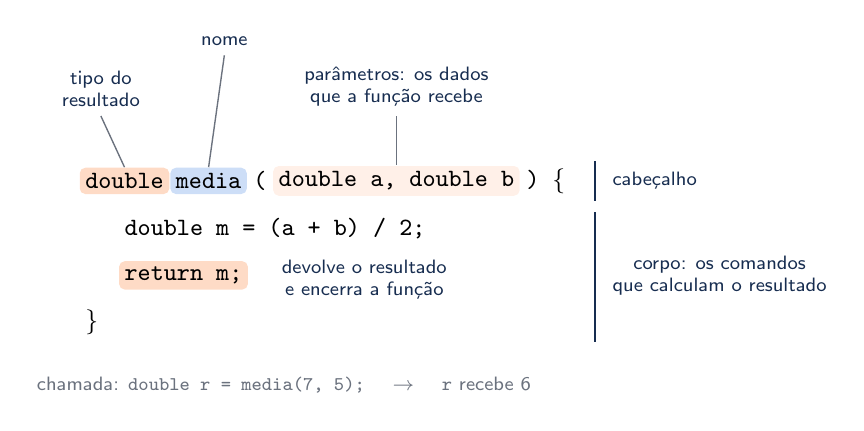
\begin{tikzpicture}
  \node[parte, fill=laranja!25, anchor=west] (tipo) at (0, 0) {double};
  \node[parte, fill=azul, anchor=west] (nome) at (tipo.east) {media};
  \node[parte, anchor=west] (ab) at (nome.east) {(};
  \node[parte, fill=laranja!10, anchor=west] (par) at (ab.east) {double a, double b};
  \node[parte, anchor=west] (fe) at (par.east) {) \{};
  \node[parte, anchor=west] (l1) at (0.5, -0.6) {double m = (a + b) / 2;};
  \node[parte, fill=laranja!25, anchor=west] (ret) at (0.5, -1.2) {return m;};
  \node[parte, anchor=west] (fim) at (0, -1.8) {\}};

  \node[expl] (e1) at ($(tipo.north)+(-0.3, 1.0)$) {tipo do\\resultado};
  \node[expl] (e2) at ($(nome.north)+(0.2, 1.6)$) {nome};
  \node[expl] (e3) at ($(par.north)+(0, 1.0)$) {parâmetros: os dados\\que a função recebe};
  \draw[guia] (e1.south) -- (tipo.north);
  \draw[guia] (e2.south) -- (nome.north);
  \draw[guia] (e3.south) -- (par.north);

  \draw[navy, line width=0.9pt] ($(fe.east)+(0.3, 0.25)$) -- ($(fe.east)+(0.3, -0.25)$);
  \draw[navy, line width=0.9pt] ($(fe.east)+(0.3, -0.4)$) -- ($(fe.east)+(0.3, -2.05)$);
  \node[expl, anchor=west] at ($(fe.east)+(0.4, 0.0)$) {cabeçalho};
  \node[expl, anchor=west] at ($(fe.east)+(0.4, -1.2)$) {corpo: os comandos\\que calculam o resultado};
  \node[expl, anchor=west] at ($(ret.east)+(0.3, -0.05)$) {devolve o resultado\\e encerra a função};
  \node[legenda] at (2.6, -2.6) {chamada: \texttt{double r = media(7, 5);} \quad $\rightarrow$ \quad \texttt{r} recebe 6};
\end{tikzpicture}
\end{document}
